\chapter{MNIST experiments}

\section{MNIST}

Jest to zbiór pokategoryzowanych odręcznie napisanych cyfr. Wszystkie obrazki są czarno-białe, rozmiaru 28x28 i wycentrowane. Zbiór składa się z 60000 danych treningowych i 10000 testowych. Zbiór ten często wykorzystywany jest w celu ekperymentowania z modelem, jednak jest na tyle mało skomplikowany, że daje jedynie poglądowe informacje. Przykładowe obrazki \ref{fig:mnist}.

\begin{figure}[h]
    \centering
    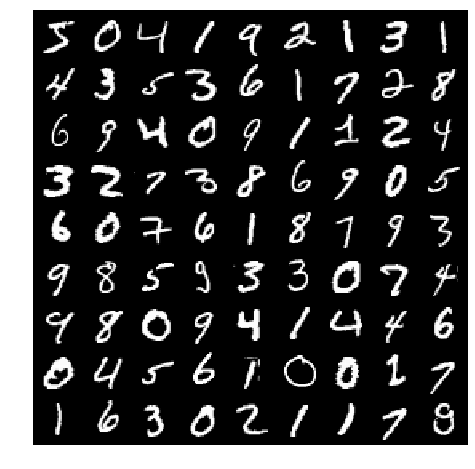
\includegraphics[width=0.5\textwidth]{mnist}
    \caption{Samples from MNIST dataset}
    \label{fig:mnist}
\end{figure}

\section{VAE}

Wyniki przy użuciu zwykłego VAE

\begin{figure}[h]
    \centering
    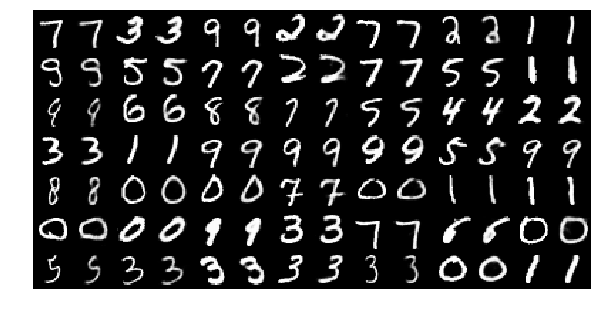
\includegraphics[width=1.0\textwidth]{mnist_recon}
    \caption{}
    \label{fig:mnist_recon}
\end{figure}

\begin{figure}[h]
    \centering
    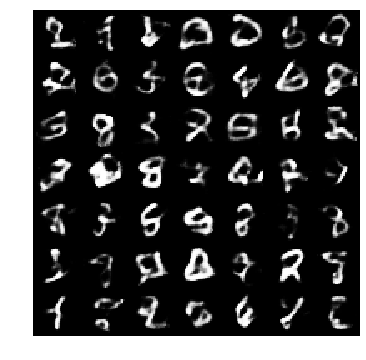
\includegraphics[width=0.6\textwidth]{images/mnist_gen.png}
    \caption{}
    \label{fig:mnist_gen}
\end{figure}

\section{Deep feature consistent variational auto-encoder}

Wyniki przy użyciu Deep feature consistent variational auto-encoder.
